\documentclass[crop=true]{standalone}
\usepackage{tikz}
\usepackage{tkz-euclide}
\usetkzobj{all}
\begin{document}

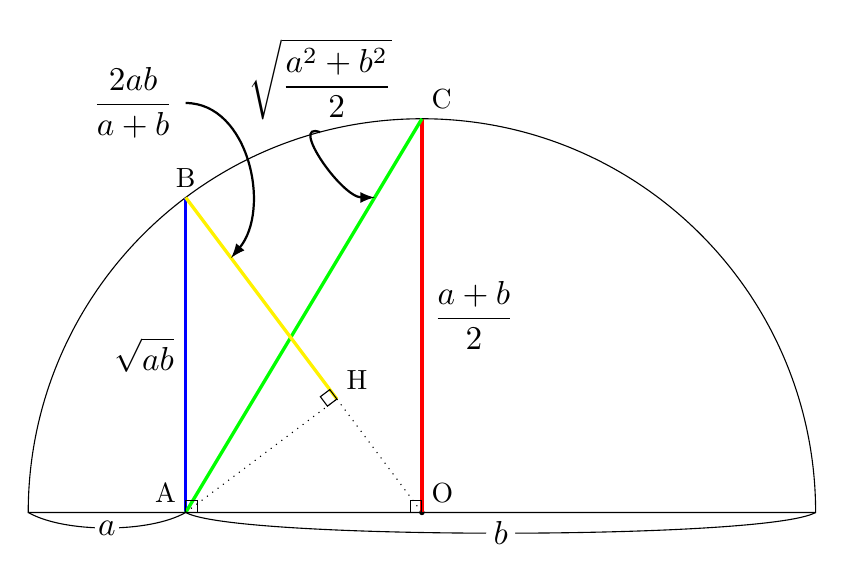
\begin{tikzpicture}[scale=5]

% 張興和. 2019. “データ分析で常用される4種類の平均の使い分け : 算術平均・幾何平均・調和平均・平方平均.” 旭川大学経済学部紀要 (78): 43–59.
% 図1 半円内の線分の長さによる4種類の平均値の大きさの表示(P.49)

  % 半径 = 1
  \def \rad{1};
  % a:b = 2:8
  \def \a{\rad * 2 * 0.2};
  \def \b{\rad * 2 * 0.8};

  % 半円
  \draw ([shift={(0,0)}]0:1) arc [radius=\rad, start angle = 0, end angle=180]--cycle;

  % 原点O
  \coordinate[label = above right:O] (O) at (0,0);
  \fill (0, 0) circle (0.2pt);
  % 点
  \coordinate[label = above left:A, scale=1.2] (A) at (-\b + \rad, 0); % 点A
  \coordinate[label = above:B, scale=1.2] (B) at (-\b + \rad, {sqrt(\a*\b)}); % 点B
  \coordinate[label = above right:C, scale=1.2] (C) at (0, 1); % 点C
  \coordinate[label = above right:H, scale=1.2] (H) at ($(B)!(A)!(O)$); % 点H
  
  % 線
  \draw[very thick, blue] (A)--(B);
  \draw[very thick, red] (C)--(O);
  \draw[very thick, green] (A)--(C);
  \draw[dotted] (A)--(H);
  \draw[very thick, yellow] (B)--(H);
  \draw[dotted] (H)--(O);
  \draw [bend left, distance = 3] (A)
    to node [fill = white, inner sep=0.2, circle, scale=1.2] {$a$} (-\rad, 0);
  \draw [bend right, distance = 4] (A)
    to node [fill = white, inner sep=0.2, circle, scale=1.2] {$b$} (\rad, 0);
 
  % 直角記号
  \tkzMarkRightAngle[size=.03](A,H,B);
  \tkzMarkRightAngle[size=.03](B,A,O);
  \tkzMarkRightAngle[size=.03](A,O,C);

  % 算術平均(arithmetic mean)
  \node(AM) at ($(C)!.5!(O)$) [right, scale=1.2, black] {$\displaystyle \frac{a + b}{2}$};
  % 幾何平均(geometric mean)
  \node(GM) at ($(A)!.5!(B)$) [left, scale=1.2, black] {$\displaystyle \sqrt{ab}$};
  % 調和平均(harmonic mean, subcontrary mean)
  \draw[-latex,thick]($(B)!-.3!(A)$)
    node[left, scale=1.2, black]{$\displaystyle \frac{2ab}{a + b}$}
    to[out=0,in=50] ($(B)!.3!(H)$);
  % 二乗平均平方根(root mean square)
  \draw[-latex,thick, black](105:\rad)
    node[above, scale=1.2]{$\displaystyle \sqrt\frac{a^2 + b^2}{2}$}
    to[out=160,in=180] ($(C)!.2!(A)$);
        
\end{tikzpicture}

\end{document}
